
\documentclass[11pt,onecolumn,a4paper,DIV=calc]{scrartcl}
\usepackage[protrusion=true,expansion=true]{microtype}
\usepackage[utf8]{inputenc}
\usepackage[T1]{fontenc}
\usepackage[ngerman]{babel}
\usepackage{graphicx}
\usepackage{wrapfig}
\usepackage{float}
%\usepackage[hyphens]{url}
\usepackage{hyperref}
\usepackage{url}
\usepackage{amsmath}
\usepackage{amssymb}
\usepackage{microtype}
\usepackage{times}
\usepackage{helvet}
\usepackage{listings}
\author{Hendric Lenz}
\usepackage{colortbl}
\usepackage{xcolor}
\PassOptionsToPackage{hyphens}{url}                      % Sorgt für URL-Umbrueche in Fusszeilen u. Literatur
%\usepackage{soul}
\renewcommand{\familydefault}{\sfdefault}
\definecolor{uhhred}{cmyk}{0,100,100,0}
\title{MvS Hausarbeit: Coloured Petri Nets}
\begin{document}

\pagenumbering{gobble}
\begin{titlepage}

\includegraphics[scale=0.3]{UHH-Logo_2010_Farbe_CMYK.pdf}
\vspace*{1cm}
\Large
\begin{center}
{\color{uhhred}\textbf{Seminararbeit}}
\vspace*{1.5cm}\\
{\LARGE \textbf{Coloured Petri Nets}}
\vspace*{2.0cm}\\
vorgelegt von
\vspace*{0.4cm}\\
Hendric Lenz 
\end{center}
\vspace*{4.9cm}

\noindent
\large
MIN-Fakultät \vspace*{0.4cm} \\
Fachbereich Informatik \vspace*{0.4cm} \\
Modul Modellierung verteilter Systeme
\end{titlepage}


\newpage


\section*{Zusammenfassung}


\newpage
\tableofcontents
\vspace{0.5cm}
\normalsize
\newpage

\pagenumbering{arabic}
\section[Allgemeines]{Allgemeines}
Etwa 19 Jahre nach der Erfindung von Petri-Netzen (PN) durch Carl Adam Petri im Jahre 1960, stellte Kurt Jensen in seiner PhD Thesis die erste Version der \textit{Coloured Petri Nets} (CPN) vor, die eine rückwärtskompatible Erweiterung zu den einfachen Petri-Netzen darstellt \cite{CPN}. Da die CPN also auf den so genannten \textit{low-level Netzen} aufbaut, sollen diese initial im Folgenden erläutert werden.\\
\newline
Ein Petri-Netz wird genutzt, um beliebig komplexe, nebenläufige und verteilte Systeme abstrakt darzustellen. Anzumerken ist hierbei, dass PN und auch CPN allgemeine Modellierungsprachen sind. Das heißt, ihr Anwendungsbereich beschränkt sich nicht auf Systeme informatischer Natur; in der Praxis finden sie zum Beispiel auch in der Wirtschaft, zur Beschreibung von Prozessen oder der Biologie Verwendung. Durch abstrakte Modellierung erlangt man mit PN ein besseres Verständnis des abgebildeten Modells und man ermittelt die Vollständigkeit und Korrektheit. Fehler in Form von Lücken oder nicht erreichbaren Zuständen werden schnell ersichtlich und sind reproduzierbar. \\
Für die Darstellung eines Netzes werden folgende Elemente definiert:
\begin{center}
\[(P,\ T,\ A,\ m_0)\] \\
\end{center}

Wobei \begin{itemize}
\item $P$ für Stellen oder auch Plätze steht.
\item $T$ für Transitionen.
\item $A$ für deren (Fluss-)Relation zueinander, also die Kanten. \\
Hierbei gilt $F \subseteq\ (P\ \times\ T)(T\ \times\ P)$, Stellen werden also stets über Kanten mit Transitionen verbunden oder anders herum, nie werden Stellen mit Stellen oder Transitionen mit Transitionen verbunden.
\item $m_0$ die Anfangsmarkierung.
\end{itemize}
Damit eine Transition schalten kann, muss auf einem davor liegenden Platz ein "Token"\ bzw. eine "Marke"\ liegen. Ist eine Transition vollzogen, werden die benötigten Marken von dem Platz entfernt. Es ist außerdem anzumerken, dass alle Mengen die für ein Petri-Netz oder ein CPN definiert werden, endlich sein müssen.\\
Petri-Netze können verschiedene Verhalten aufweisen. Zuallererst sind PN immer geordnet, was bedeutet, dass a immer vor b eintritt. Außerdem können sie nicht-deterministisch sein. Eine Stelle kann über zwei gleichwertige, nachfolgende Transitionen verfügen und es ist nicht festgelegt, welche der beiden Transitionen im nächsten Schritt schaltet. Des Weiteren können PN nebenläufig sein, was bedeutet, dass mehrere Transitionen gleichzeitig innerhalb eines Netzes unabhängig voneinander schalten können. 
Darüber hinaus weisen Petri-Netze eine Reihe von Eigenschaften auf. Ein Netz:
\begin{itemize}
\item terminiert, kommt also immer in einen sogenannten \textit{toten Zustand}.
\item ist deadlockfrei oder schwach lebendig, wenn es immer mindestens eine Transition gibt, die schalten kann.
\item ist lebendig, wenn alle Transition unter jeder Markierung aktivierbar sind.
\end{itemize}
\begin{figure}[h]
\center
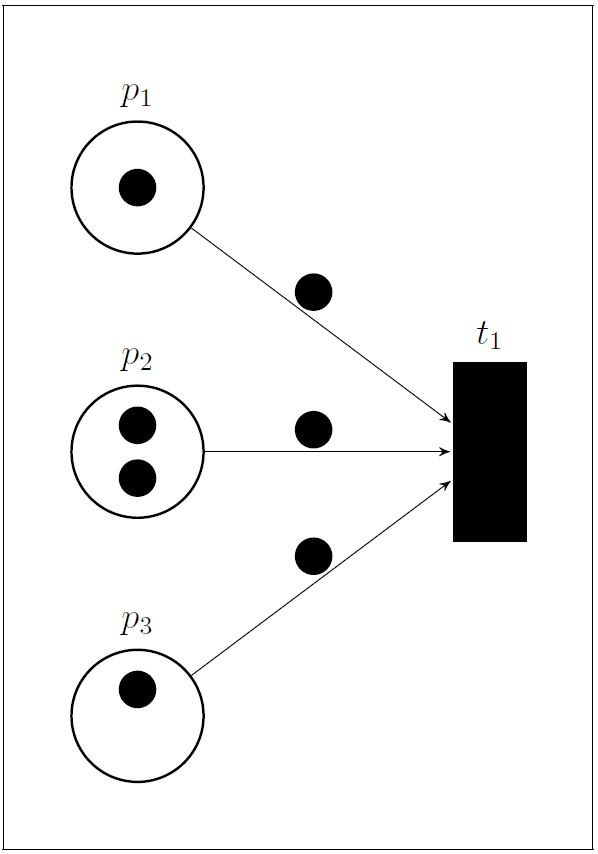
\includegraphics[scale=0.4]{netz1.PNG} \\
\caption{Petri-Netz ohne gefärbte Marken}
\end{figure}
Angenommen, Abbildung 1 beschreibt ein Lager, welches in $p1$ Schrauben enthält, in $p2$ Nägel und in $p3$ Muttern, so sind die Marken auf den entsprechenden Plätzen vorerst gleichwertig und müssen durch eine zusätzliche Beschriftung kenntlich gemacht werden. Es liegt also nahe, unterschiedliche Marken unterschiedlich zu kennzeichnen. Hierdurch und mittels Faltung, kann das Netz aus Abbildung 1 vereinfacht werden. Das neue Netz wird in Abbildung 4 als CPN dargestellt.\\

\begin{figure}[h]
\center
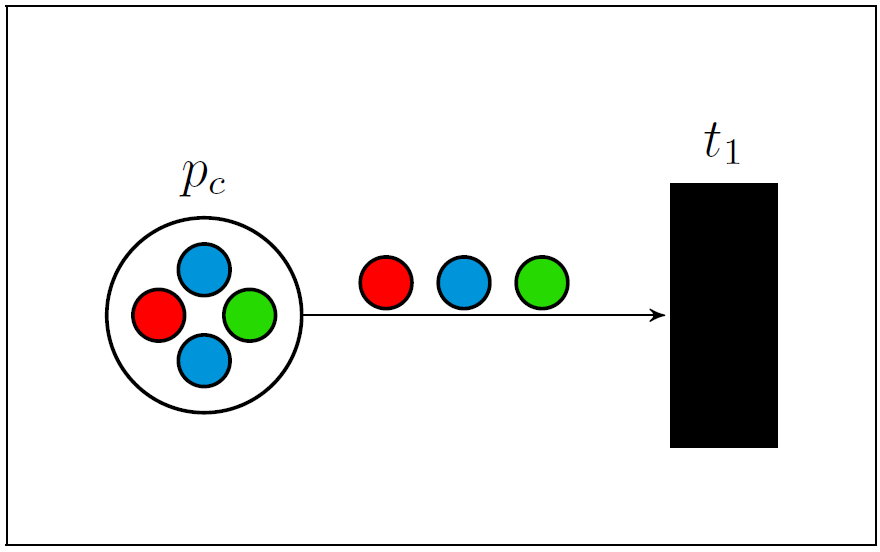
\includegraphics[scale=0.4]{netz2.PNG}
\caption{Dasselbe Netz als CPN}
\end{figure}

\subsection{Formale Definition: CPN}
Mit CPN erweiterte Kurt Jensen \cite{CPN1} 1979 die PN um folgende Attribute:
\begin{itemize}
\item $\Sigma$ stellt die Menge aller Farben dar. Diese namensgebene Erweiterung erlaubt eine Unterscheidung von Marken.
\item $V$ bezeichnet die Menge aller Variablen
\item $N$ ist die Knotenfunktion. Sie verbindet eine Kante mit zwei Stellen, wobei eine Stelle die Quelle und die andere das Ziel ist.
\item $C$ ist die Farbenfunktion. Sie bindet an jede Stelle eine bzw. mehrere lokal akzeptierte Farben.
\item $G$ ist die Guardfunktion. Diese Funktion fügt jeder Kante einen boolschen Wert hinzu, bei der alle Variablen vom Typ $\Sigma$ sind. Die Beschriftung wird bei Kanten, die immer zu $true$ auswerten nicht abgebildet.
\item $E$ ist die Kantenfunktion. Sie gibt an, dass eine Kantenfunktion aus \textit{Multiset} den angrenzenden Stellen auswerten muss. 
\item $I$ ist die Inititialisierungsfunktion.
\end{itemize}
Bei CPN handelt es sich des Weiteren um ein \textit{höheres Petri-Netz} oder auch \textit{high-level net}. Diese zeichnen sich durch eine Kombination von Programmiersprachen und low-level Netzen aus. Es können also beispielsweise Schleifen, Zähler oder Funktionen vorkommen. Weitere Beispiele für höhere Netze sind das Predikatennetz und das Transitionsnetz.

\newpage
\subsection{Verifikation}
Verifikation kann durch zwei Verfahren erreicht werden. Zum einen gibt es die Methode des Markierungsgraphen, auch \textit{State-Space-Method} genannt. 
\begin{wrapfigure}{l}{0.6\textwidth}
\begin{center}
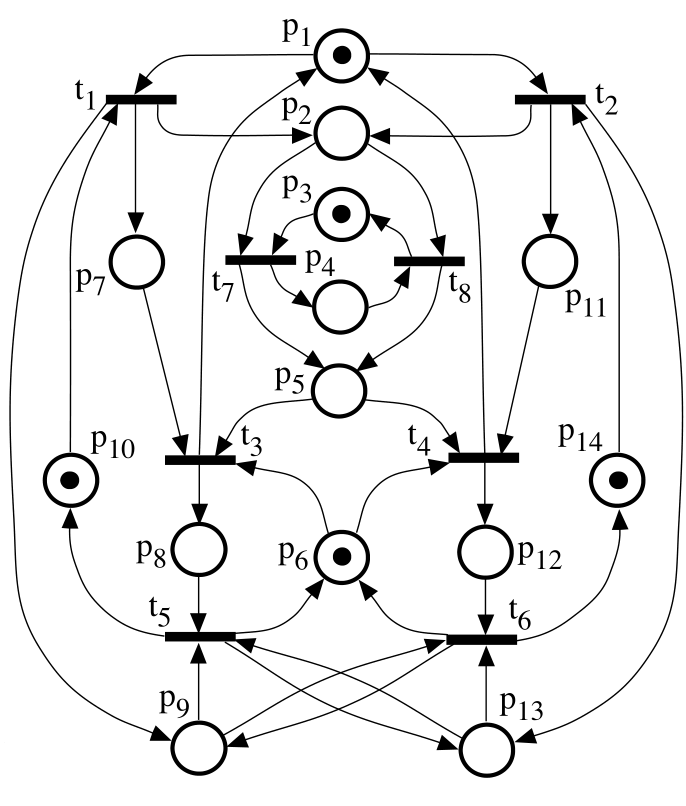
\includegraphics[scale=0.35]{netz3.PNG}\caption{Ein low-level Petri-Netz}
\end{center}
\end{wrapfigure}
Hier werden, ausgehend von einer Anfangsmarkierung \\(meistens $m_0$), alle erreichbaren Markierungen als gerichteter Graph dargestellt. Eine Markierung bezeichnet bei Petri-Netzen einen Zustand des Modells. Abbildung 3 und 4 zeigen ein Petri-Netz und den dazugehörigen Markierungsgraphen.
Ein Problem dieser Methode ist das sogenannte \textit{State-explosion problem}. Ab einer gewissen Komplexität des Netzes steigt die Anzahl der Markierungen stark an, was den resultierenden Graphen zuerst unübersichtlich macht und außerdem eine hohe Rechenzeit benötigt. \\
Die zweite Möglichkeit zur Verifikation sind Invarianten. Invarianten bezeichnen Werte, die vor und nach dem Ausführen, in diesem Fall von Transitionen, gleich bleiben bzw. gelten. 


\begin{figure}[h]
\center
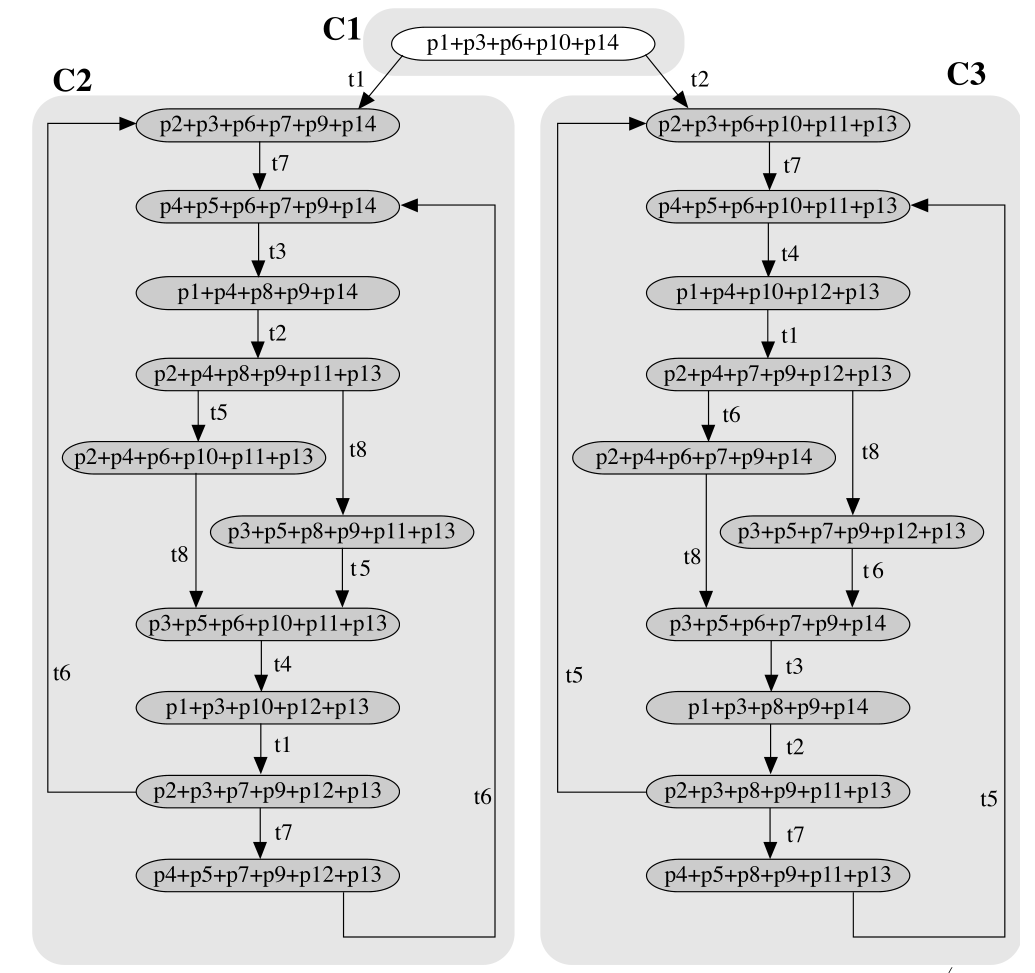
\includegraphics[scale=0.4]{graph1.PNG}
\caption{Der zu Abb. 3 gehörige Markierungsgraph}
\label{graph}
\end{figure}
\newpage

\section{Non-Hierarchische CPN}
Um die verschiedenen Typen von CPN verständlich zu erklären, werden sie folgend alle anhand eines Beispielprotokolls dargestellt. Es handelt sich dabei um ein Protokoll, welches aus dem Transport-Layer des OSI-Schichtenmodells stammt. Es besteht aus einem Sender, einem Empfänger und einem leicht unzuverlässigen Netzwerk, welches die beiden anderen Komponenten verbindet. Es kann also passieren, dass Pakete, die vom Sender abgeschickt werden durch Verlust oder Überholen anderer Pakete nicht korrekt beim Empfänger eintreffen. Um die Reihenfolge der Pakete zu überschauen und dafür zu sorgen, dass ein Paket nur genau ein mal beim Sender eintrifft, werden die Pakete mit Indizes versehen, es werden Acknowledgements verschickt, sowie Sendungen wiederholt.\\
\begin{figure}[h]
    \centering
    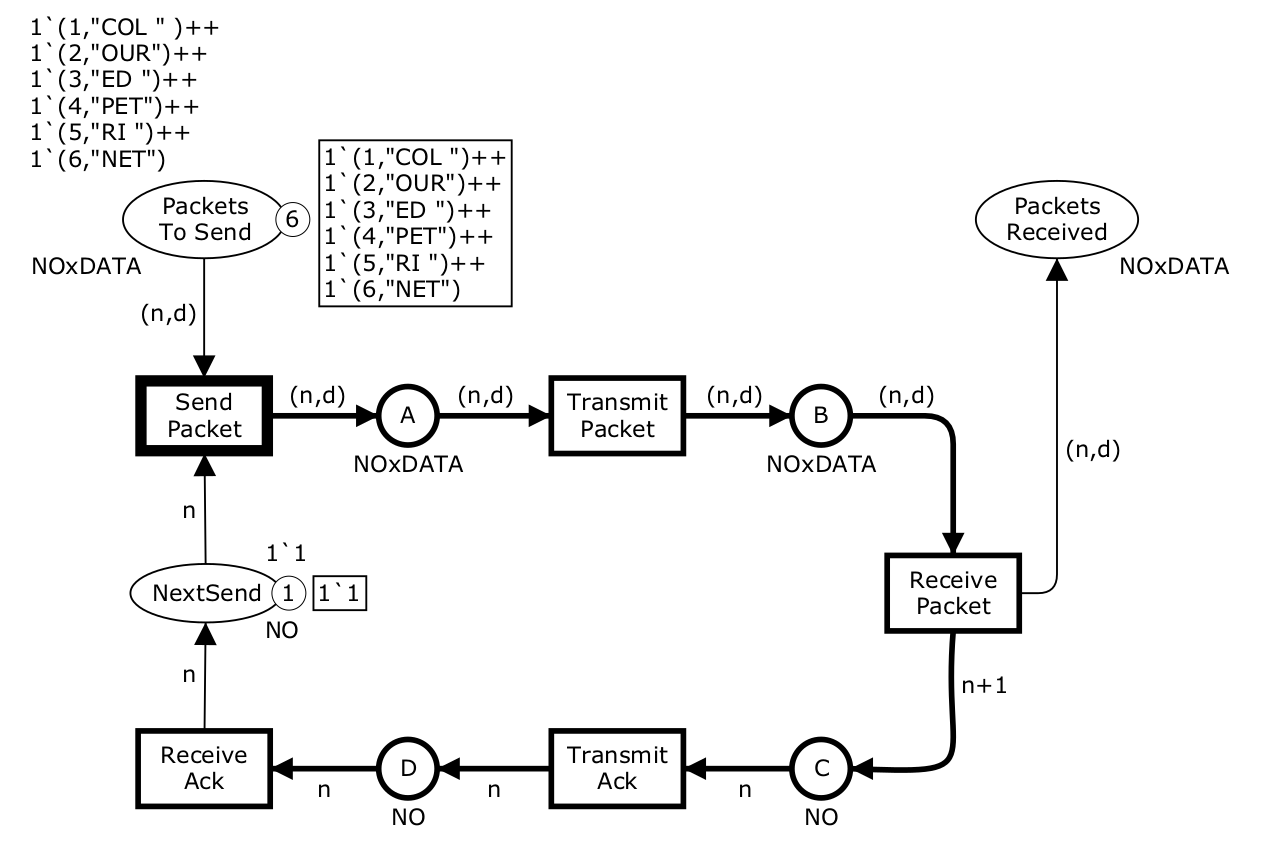
\includegraphics[scale=0.28]{non1.png}
    \caption{Non-hierarchisches Netz in der Anfangsmarkierung \texttt{M0}}
    \label{m0}
\end{figure}
Verschiedene Zustände innerhalb von verteilten Netzen werden \textit{Markierungen} genannt. Die Anfangsmarkierung \texttt{M0} bezeichnet den Startzustand eines Netzes. Schalten nun die ersten Transitionen in einem ersten Schritt, erreicht man die nächste Markierung \texttt{M1}.
In Abbildung 5 zu sehen ist das Transport Protokoll im Startzustand. Zu sehen sind 7 Plätze, welche typischerweise als Rechtecke dargestellt werden und 5 Transitionen, als Kreise abgebildet. Verbunden werden diese Komponenten mit Kanten, als gerichtete Pfeile gezeigt.\\
\newline
Äußerst links-oben zu sehen sind die Pakete, welche vom Sender zum Empfänger geschickt werden sollen. Ein Paket besteht in diesem Fall aus zwei Variablen vom Typ Integer und String. Der Integer stellt die Laufnummer des Paketes dar und der String die Nutzlast des Pakets. Die Pakete finden sich außerdem in Abbildung 5 im Speicher \texttt{Packets To Send} wieder, wo die Anzahl der dort abliegenden Pakete rechts in Form eines Integers in einem Kreis beschrieben wird.\\
Die Symbole \texttt{'} und \texttt{++} erzeugen ein \textit{Multiset}, was in diesem Fall aus den sechs Packeten besteht. Ein Multiset ähnelt einem Set, nur können Pakete mehrfach vorkommen. Die Häufigkeit des Vorkommens wird durch den Integer vor dem \texttt{'} beschrieben.\\
Transitionen stellen die möglichen Aktionen innerhalb eines Netzes dar und werden über Kanten mit Plätzen verbunden, hier dargestellt als gerichtete Pfeile. Beschriftet werden diese mit den von der Transition akzeptierten Colours, im Fall von Transition \texttt{Send Paket} sind das \texttt{n} für Number, wieder in Form von Integer und \texttt{d} für Data in Form eines String.\\
Auch neben den Plätzen sind die aktzeptierten Token-Farben verzeichnet. Platz \texttt{A} erlaubt nur eine Vereinigung der Farben \texttt{NO} und \texttt{DATA}, hier als \\\texttt{NOxDATA} dargestellt. Hierbei ist \texttt{NO} wieder vom Typ Integer und \texttt{DATA} vom Typ String.\\
\newline
Im ersten Schritt wird geprüft, welche der Transitionen schalten kann. Auf \texttt{NextSend} liegt ein Token der Farbe \texttt{1} ab und erfüllt somit alle Bedingungen für die Transition \texttt{Send Paket}. Das Token auf \texttt{NextSend} gibt die Indexnummer des Pakets vor, welches als nächstes gesendet werden soll. 
In \texttt{Send Packet} nimmt das erste Paket vom Speicher und erzeugt ein identisches Token auf Platz \texttt{A}. Nach diesem Schritt wird Markierung \texttt{M1} erreicht. Auf dem Startspeicher \texttt{Packets To Send} liegen jetzt nur noch 5 Pakete ab, auf Platz \texttt{A} eines.\\
Eine Markierung später wird die Transition \texttt{Receive Packet} aktiviert. Diese erzeugt eine Marke mit der aktuellen Laufnummer und dem dazugehörigen String und legt sie auf dem Zielspeicher ab. Außerdem wird eine weitere Marke erzeugt, welche auf Platz \texttt{C} abgelegt wird. Diese besteht, wie an der Kennzeichnung an der Kante zu \texttt{C} beschrieben, nur noch aus der Laufnummer. Sie wird außerdem um 1 erhöht, was dazu führt, dass eine 2 nach 2 weiteren Schritten auf dem Platz von \texttt{NextSend} abliegt und somit den Durchlauf von Paket 2 auf dem Startspeicher anstößt.
\begin{figure}[H]
    \centering
    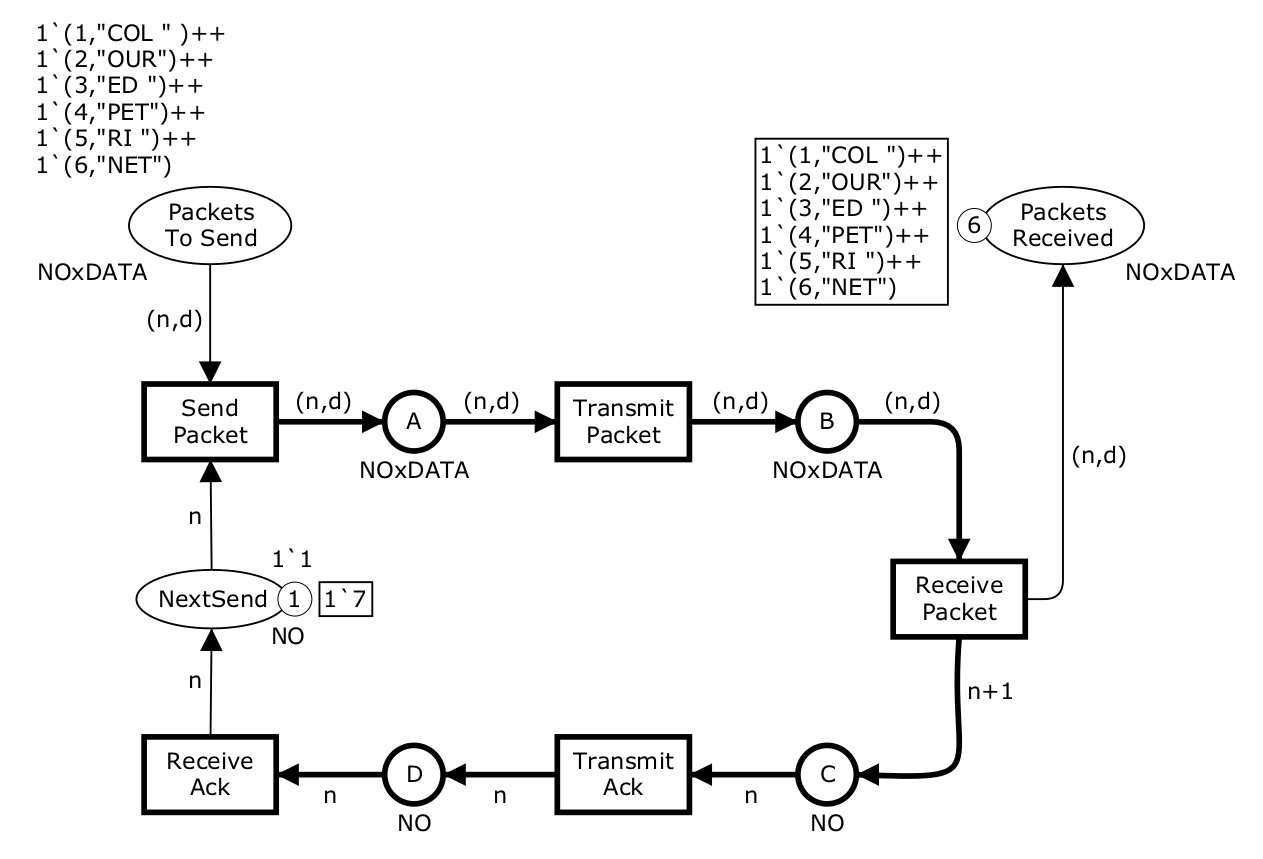
\includegraphics[scale=0.28]{non30.png}
    \caption{Das Netz in seinem Endzustand \texttt{M30}}
    \label{m30}
\end{figure}
Alle Pakete sind nach 30 Schritten beim Empfänger angekommen. In der letzten Markierung wird die sogenannte \textit{Tote Markierung} erreicht, wo keine weitere Transition aktiviert werden kann.\\
Dieses Modell eines CPN weist nicht die typischen Eigenschaften wie Nicht-Determinismus oder Konflikt auf. Ein neues, leicht verändertes Netz zeigt diese Eigenschaften in Abbildung \ref{fig:modified}\ aber auf.
\begin{figure}[H]
    \centering
    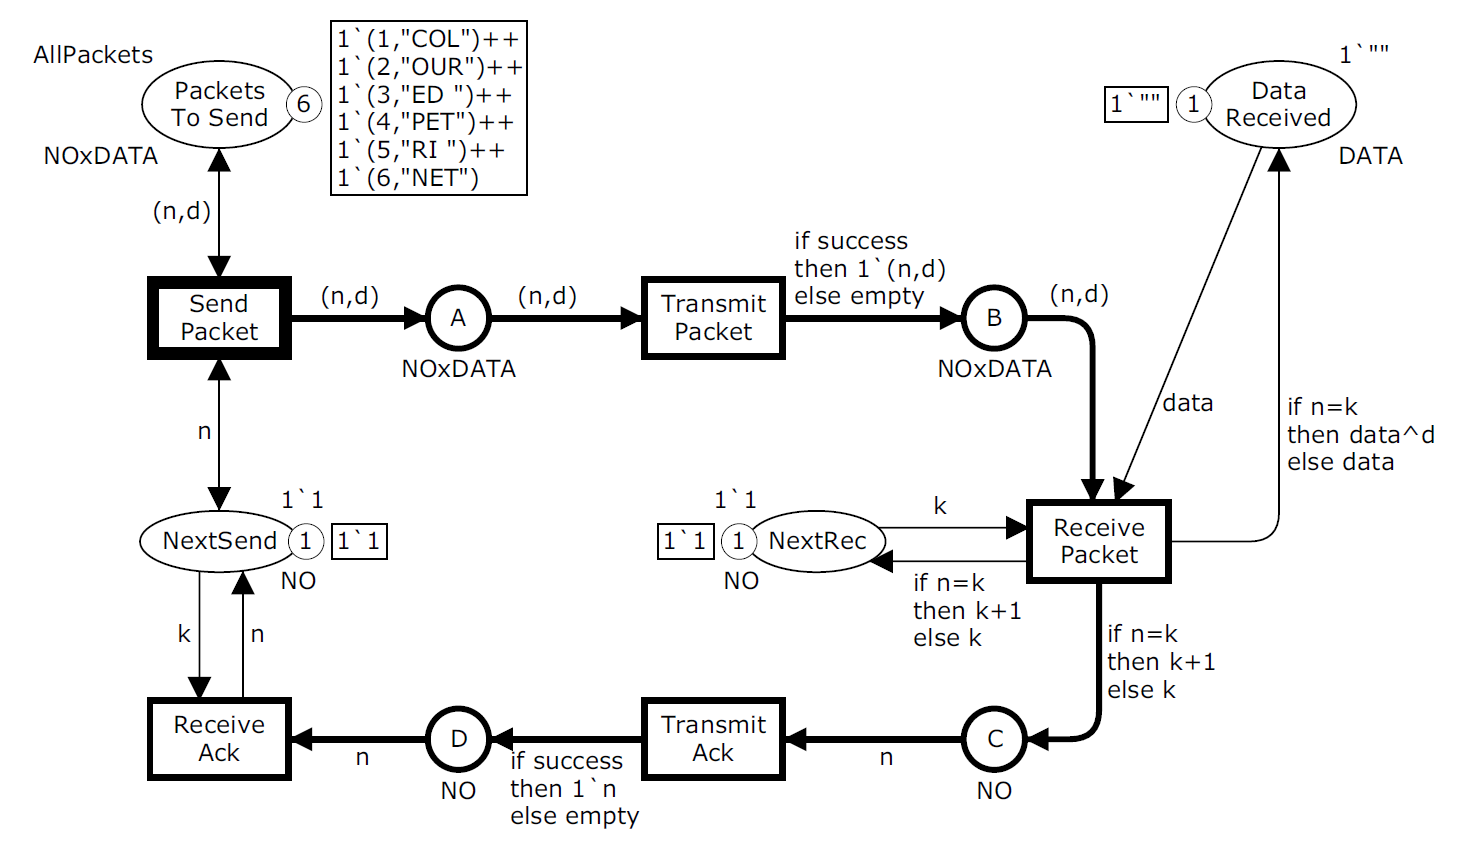
\includegraphics[scale=0.4]{non2_1.PNG}
    \caption{Modifizierte Version des ersten Netzes}
    \label{fig:modified}
\end{figure}
Im Gegensatz zum vorherigen Netz nimmt der Empfänger hier ausschließlich den \texttt{DATA} Teil des Pakets entgegen. Außerdem liegt auf dem Zielspeicher bereits ein leerer String ab, an welchen die \texttt{DATA} Inhalte der Pakete fortlaufend angehängt werden. Die Laufnummer dagegen wird beim Platz \texttt{NextRec} mit der erwarteten Laufnummer verglichen. Stimmen die Integers überein, wird genau wie im ersten Netz die Laufnummer um eins erhöht und über das Netz weiter bis \texttt{NextSend} geleitet. Sollte dies allerdings nicht der Fall sein, wird die Nummer nicht erhöht und löst bei \texttt{NextSend} das erneute Senden des vorherigen Pakets aus.\\
Des Weiteren verfügt die Transition \texttt{Transmit Packet} nun über einen boolschen Wert, der angibt, ob das Paket erfolgreich übermittelt wurde. Sollte dies der Fall sein, wird die Marke bzw. das Paket auf \texttt{A} entfernt und eine neue Marke wird auf Platz \texttt{B} erzeugt, wobei diese neue Marke zu dem zuvor entfernten Paket identisch ist. Sollte das Paket dagegen verloren gehen wird die Marke wiederrum von \texttt{A} entfernt, jedoch wird keine neue Marke auf Platz \texttt{B} erzeugt.\\
Die selbe boolsche Funktion wird auch nach der Transition \texttt{Transmit Ack} gefunden, wo die Laufnummer wieder im Netzwerk verloren gehen kann. Die Funktionsweise ist dieselbe wie bei \texttt{Transmit Packet}.\\
Das neue Netz erlaubt außerdem Nebenläufigkeit. Das heißt, dass mehrere Pakete gleichzeitig und unabhängig voneinander im Netz verkehren können. Der Empfänger ist sogar dazu im Stande, bereits empfangene Pakete wieder abzuweisen ohne das deren Nutzlast, in Form des String, an den String im Zielspeicher angefügt wird.


\subsubsection*{Guards}

Guards stellen eine Bedingung in Form eines boolschen Ausdrucks dar, die bestimmen, ob eine Transition schaltet oder nicht. In dem Beispiel stellten die boolschen Ausdrücke eine erfolgreiche Übermittlung über das Netzwerk dar. Oft werden Guards aber auch genutzt, wenn verschiedene Systeme auf gemeinsame Ressourcen zugreifen müssen. Ist eine Ressource vorhanden, kann ein Prozess auf sie zugreifen. Sollte dies nicht der Fall sein, muss der Prozess auf eine Freigabe der Ressource warten. Oft werden statt boolscher Werte an den Transitionen auch Modelle mit Marken verwendet, um das Netz homogener darzustellen. In der CPN ML-Sprache werden vereinfachend aber boolsche Werte genutzt. %TODO: ML

\section{Hierarchische CPN}
Petri-Netze werden ab einer gewissen Komplexität schnell unübersichtlich. Um große Netze erfassbar zu machen wurde die Modulisierung, vergleichbar mit Objekten aus objektorientierten Programmiersprachen, vorgestellt. Das im vorherigen Kapitel vorgestellte Netz kann in seine Einzelteile zerlegt werden: Sender, Empfänger und Netzwerk. Das resultierende Netz erlaubt ein schnelles Verständnis, jedoch keine detaillierte Einsicht in die einzelnen Komponenten. Dieses Level von Abstraktion nennt man Protokoll-Modul.
\begin{figure}[H]
    \centering
    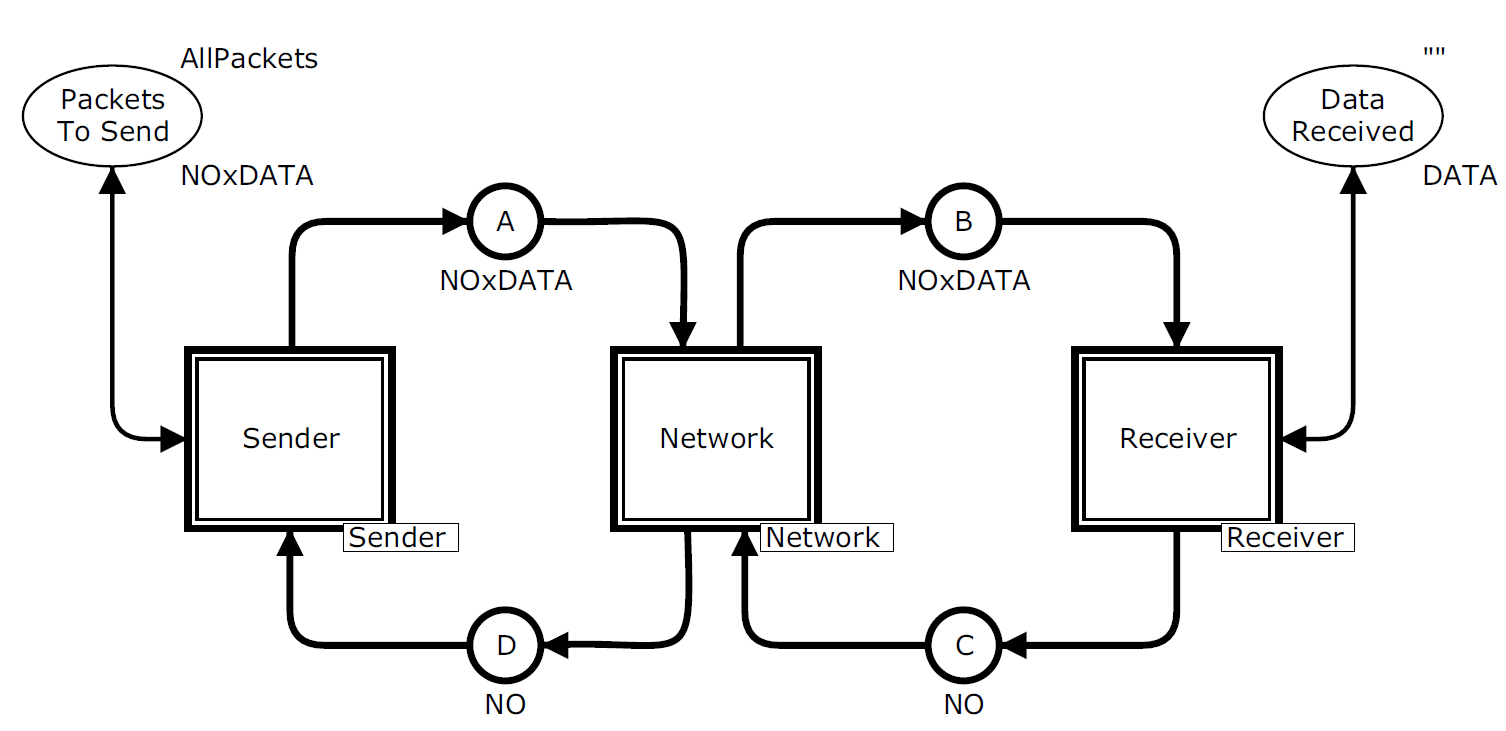
\includegraphics[scale=0.4]{hier1.PNG}
    \caption{Das Protokoll auf seine Komponenten heruntergebrochen}
    \label{fig:Hier1}
\end{figure}
Jedes Modul, hier als doppelt gerahmte Rechtecke dargestellt, verfügt über In- und Outputsockets, über welche mit anderen Komponenten kommuniziert wird. Im Falle des Beispiels übernehmen die Plätze \texttt{A} bis \texttt{D} die Rolle der Sockets.\\
\newline
Um das Modell weiter zu vereinfachen, werden die beiden Transitionen im Netzwerk zusammengefasst. Der Unterschied lag bei den akzeptierten Marken: \texttt{Transmit Packet} akzeptiert Marken des Colourset \texttt{NOxDATA}, wogegen \texttt{Transmit Ack} nur Marken im Integerbereich zulässt. Man kann also ein neues Colourset anlegen, welches \texttt{NOxDATA} und \texttt{NO} akzeptiert. Das neu entstandene Modul wird \texttt{Transmit Module} genannt und tritt nun in zwei \textit{Instanzen} auf.\\
\newline
Man kann die Relationen zwischen Modulen als gerichteten Graphen darstellen, was den hierarchischen Netzen seinen Namen verleiht. Jedes Modul wird durch einen Knoten dargestellt und jede substituierte Transition als eine Kante. 
\begin{figure}[H]
    \centering
    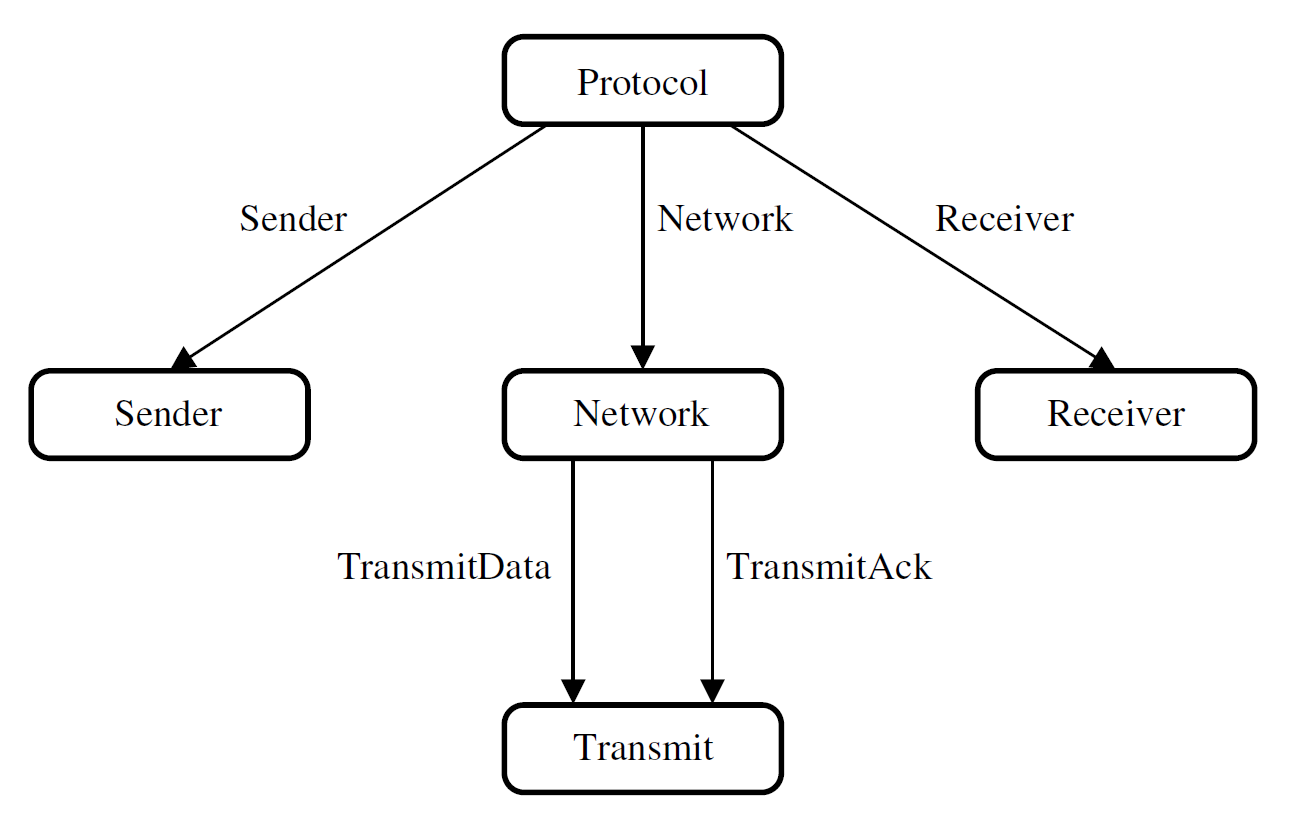
\includegraphics[scale=0.46]{hier3.PNG}
    \caption{Modulhierarchie des Netzes}
    \label{hierarchy1}
\end{figure}
Es ist ebenfalls möglich, das Netz als einen gerichteten Baum darzustellen, wo jeder Knoten eine Instanz und jede Substitution eine Kante ist. 
\begin{figure} [H]
    \centering
    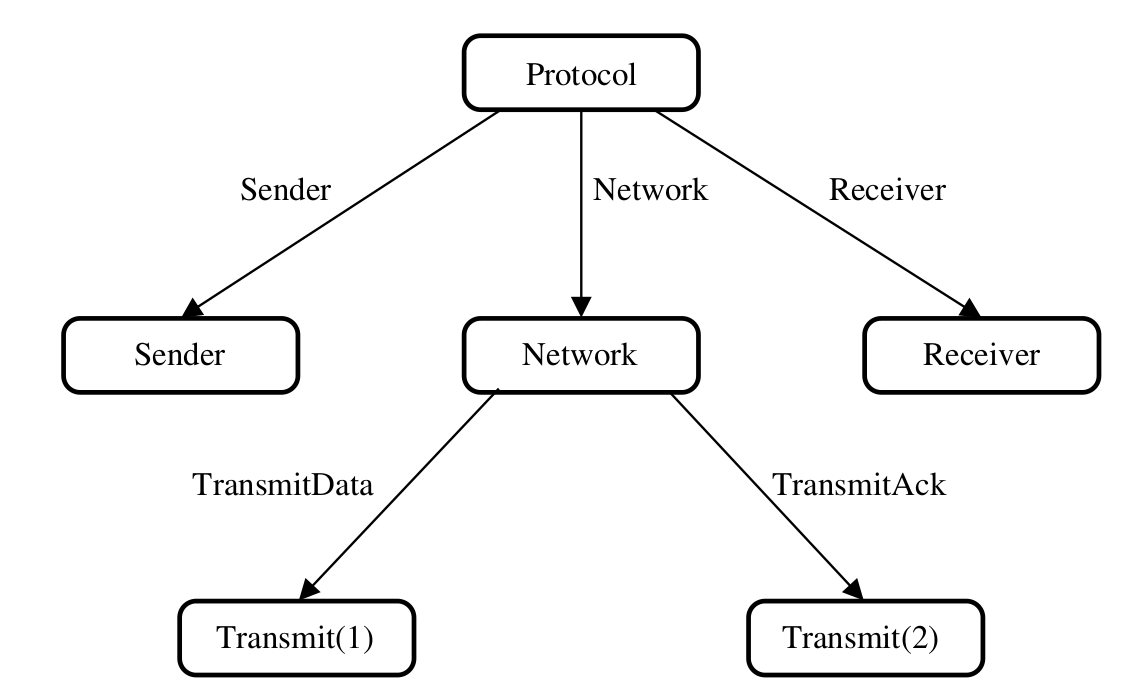
\includegraphics[scale=0.3]{hier.png}
    \caption{Instanzhierarchie des Netzes}
    \label{fig:my_label}
\end{figure}
Neben der vereinfachten Darstellung von komplexen Netzen bringen die hierarchischen Netze zwei weitere Vorteile mit sich: Parametrisierung von Modulen und Faltung.

Das Beispielnetz wird nun um einen Empfänger erweitert. \texttt{Receiver 1} und \texttt{Receiver 2} erhalten die Netzwerkplätze \texttt{A} bis \texttt{D}, jeweils mit der Empfängernummer erweitert. Die Netzwerkplätze treten also doppelt auf - für jeden \texttt{Receiver} ein mal.
Bei \texttt{Receiver 1} und \texttt{Receiver 2} handelt es sich um sogenannte \textit{Substitutionstransitionen}. Hier handelt es sich um die vereinfachten Komponenten, also beispielsweise sind in Abbildung \ref{fig:Hier1} der Sender, das Netzwerk und der Empfänger, welche ebenfalls Substitutionstransitionen sind.\\
Um das Netzwerk wieder zu vereinfachen, werden die akzeptierten Farben wieder so erweitert, dass es die Pakete beider Receiver verarbeiten kann. Hierfür werden alle Pakete um die Nummer des jeweiligen Receivers erweitert, sodass zwischen ihnen unterschieden werden kann. Die Definition der akzeptierten Farben ist in Abbildung \ref{fig:para1} zu sehen.
\begin{figure}[H]
    \centering
    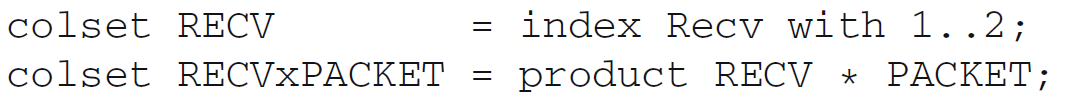
\includegraphics[scale=0.55]{para1.PNG}
    \caption{Das Netzwerk akzeptiert nun Pakete an und von Receiver 1 bis 2}
    \label{fig:para1}
\end{figure}
Diese neue Schreibweise bringt den Vorteil mit sich, dass statt\\ \texttt{Receiver 2} eine Variable eingesetzt wird, welche der Anzahl der Empfänger entspricht. Es ist also mit wenig Umstand möglich, mehrere Empfänger dynamisch, jedoch nicht zur Laufzeit, zu implementieren.

\begin{figure}[H]
    \centering
    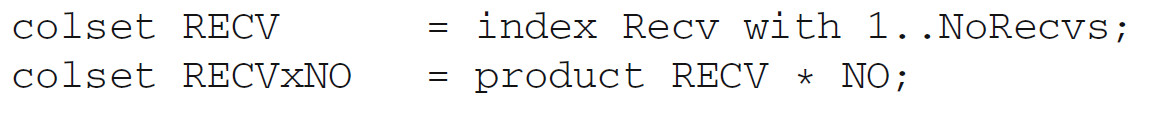
\includegraphics[scale=0.53]{para2}
    \caption{Anstelle von (Receiver) 2 steht nun die Variable \texttt{NoRecvs}}
    \label{fig:para2}
\end{figure}

Es ist folgend nicht mehr notwendig, für jeden Receiver je einen von jeden Netzwerkplätzen zu haben. Diesen Prozess nennt man \textbf{Faltung}.
%TODO: Abbildung

\section{Timed-CPN}
Timed CPN dienen der Verifizierung von Netzen, bei denen es neben der Korrektheit und Vollständigkeit auch um das richtige Timing von Prozessen geht. Performanz, maximale und durchschnittliche Warte- und Durchlaufzeiten können so festgestellt werden. 
Hierfür kann die gefärbte Marke über einen zusätzlichen Wert verfügen, einen Zeitstempel. Des Weiteren verfügen timed CPN über eine globale Uhr. Ein Zeitstempel gibt an, wann eine Marke wieder bereit ist, von der nachfolgenden Transition genutzt zu werden.
\begin{figure}[H]
    \centering
    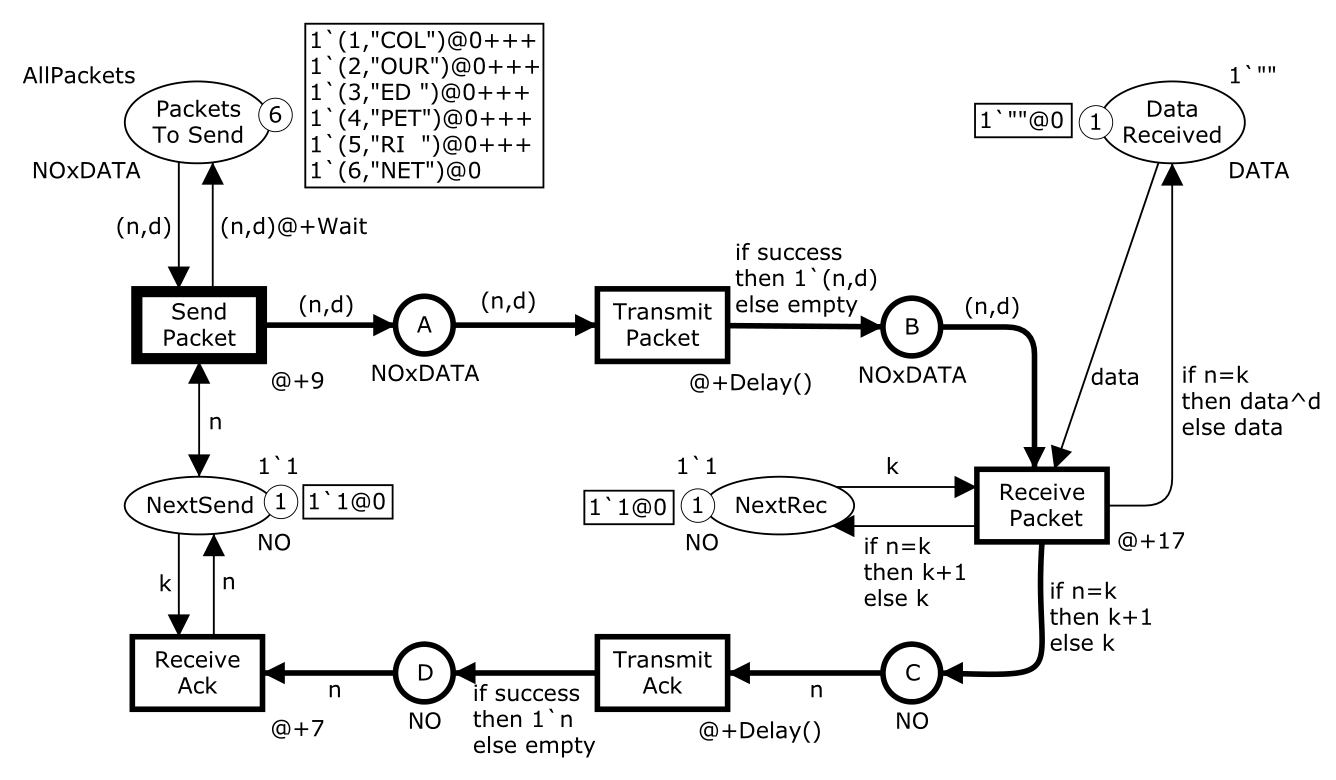
\includegraphics[scale=0.35]{tim0.PNG}
    \caption{Timed CPN in $m_0$}
    \label{fig:tim0}
\end{figure}


In Abbildung \ref{fig:tim0} ist das Transport-Layer Protokoll zu sehen, dieses mal mit Zeit-Werten, welche mit einem \texttt{@} versehen sind. Außerdem sind in \texttt{Packets To Send} die verschiedenen Tokens zu sehen, auch hier alle mit einem\texttt{@} versehen sowie dem Zeitwert, hier noch mit 0 gekenntzeichnet.\\
Schaltet nun die einzig verfügbare Transition \texttt{Send Packet}, wird, vorgegeben durch \texttt{NextSend}, das erste Paket mit der Indexnummer 1 und dem Zeitstempel 0 vom Speicher genommen. Dem Token wird ein Zeitwert von +9 hinzugezählt, was den Zeitstempel von \texttt{(1,"COL")} logischerweise zu 9 werden lässt. Das Paket sieht nun so aus: \texttt{(1,"COL")@9}. \\
Die Transition \texttt{Send Packet} legt das gerade empfangene Paket jedoch direkt wieder auf den Speicher zurück, wie die Kante zurück nach \texttt{Pakets To Send} erkennen lässt. Außerdem wird dabei ein Zeitwert von 100 Einheiten auf den Zeitstempel des Pakets hinzugerechnet, was zum einen dazu führt, dass der entsprechende Wert nun 109 beträgt und zum anderen dass das Paket erst wieder gesendet werden kann, wenn die globale Uhr 109 erreicht und alle anderen Bedingungen erfüllt sind. 
Das zweite Paket im Speicher dagegen besitzt immer noch den Zeitstempel 0 und kann deswegen sofort gesendet werden, wenn die Acknowledge-Meldung des ersten Pakets von Zeit 109 ankommt. Sollte die Acknowledge Meldung auf dem Weg zurück zum Sender, bedingt durch Verzögerungen im Netzwerk, länger brauchen als 109 Zeiteinheiten, wird das erste Paket erneut versendet und auf eine rechtzeitige Ack-Meldung gewartet.\\
\newline
Die Transition \texttt{Transmit Packet} verfügt über eine Funktion \texttt{Delay()} welche einen zufälligen Zeitwert zwischen 25 und 75 auf den Stempel des aktuellen Pakets hinzurechnet. Hiermit werden eventuelle Verzögerungen innerhalb eines Netzes simuliert, wodurch die eben beschriebene Wartezeit überschritten werden kann und ein erneutes Senden des Paketes veranlasst wird. Über die gleiche Funktion verfügt die Transition \texttt{Transmit Ack}. Diese Funktion macht das Timed CPN des Weiteren nicht deterministisch, da bei jedem Durchlauf des Petri-Netze andere Werte im Delay gewählt werden könnten. Andere Transitionen wie \texttt{Receive Packet} und \texttt{Receive Ack} dagegen, rechnen einen festen Wert auf den Zeitstempel des jeweiligen Paketes hinzu.

\section{CPN-Tools}
CPN Tools ist ein frei zugängliches Programm, mit welchem das Erstellen und Editieren, sowie das Simulieren und Analysieren von CPN auf allen gängigen Betriebssystemen möglich ist. Angeblich wird das Programm von mehr als 8000 Usern in 140 Ländern genutzt.\\
Über eine grafische Oberfläche können verschiedene Elemente eines CPN per \textit{drag-and-drop} in ein \textit{Workspace} gezogen werden und beschriftet oder eingefärbt werden, sodass auch komplexere Netze übersichtlich bleiben. \\
Die Simulation bzw. Analyse eines Netzes kann unter Umständen viel Zeit und Rechenleistung in Anspruch nehmen, wenn das Programm jede mögliche Abfolge von Transitionen innerhalb eines CPN berechnet.

\begin{figure}
    \centering
    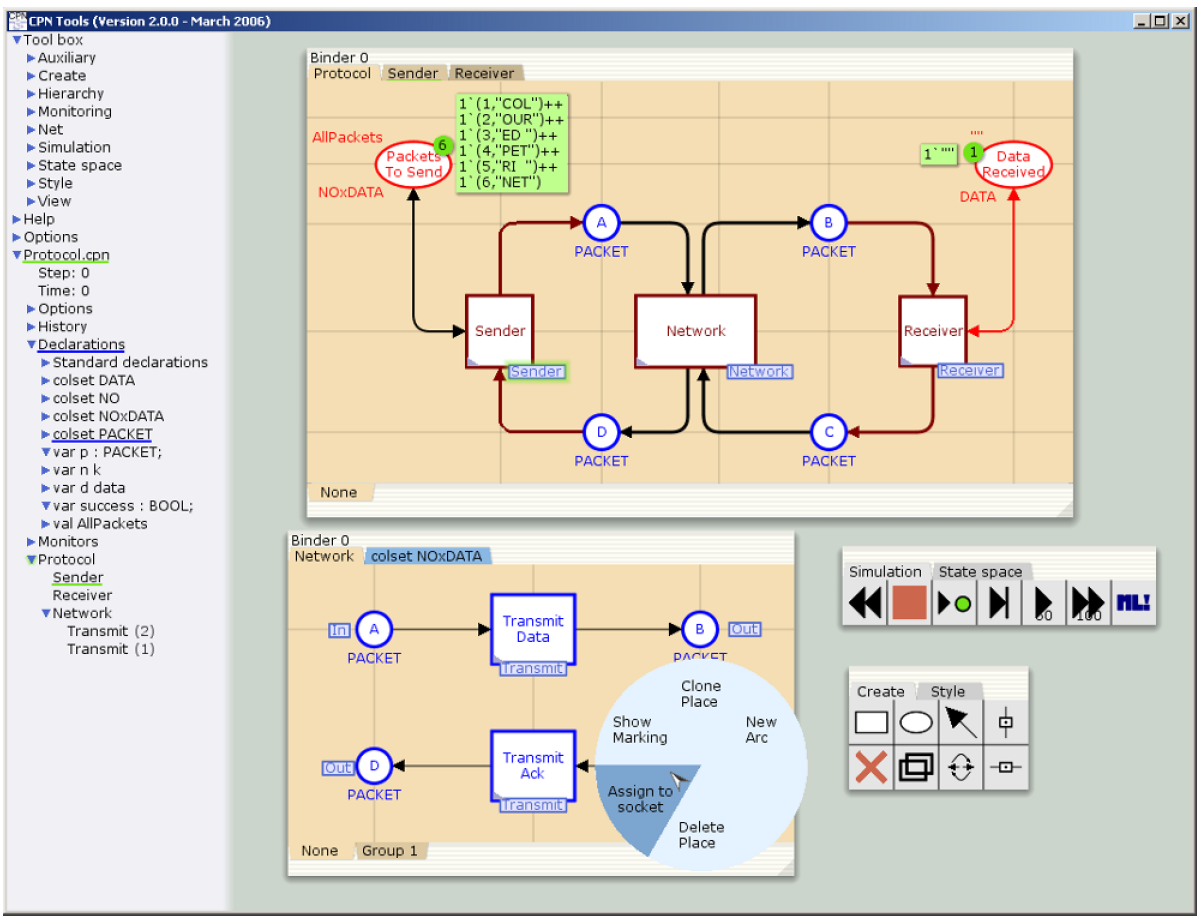
\includegraphics[scale=0.5]{tool.PNG}
    \caption{Screenshot von CPN Tools}
    \label{fig:tool}
\end{figure}

\newpage
\begin{raggedright}% schaltet Blocksatz ab, erzeugt ein stimmigeres Schriftbild im Literaturverzeichnis
\label{sec:literaturverzeichnis}
\begin{thebibliography}{Quellen}
  \bibitem{CPN} Kurz Jensen, Lars M. Kristensen - Coloured Petri Nets, Modelling and Validation of Concurrent Systems; Springer
    \bibitem{CPN1} Kurt Jensen - An Introduction to the Theoretical Aspects of Coloured Petri Nets, Paper, Computer Science Department, Aarhus University
    \bibitem{MvS} Daniel Moldt - Modellierung verteilter Systeme, Vorlesung, Foliensatz Nr. 7 - Beschränktheit, 2016
    \bibitem{Petri} Adam Petri, Wolfang Reisig - Petri Net \url{http://www.scholarpedia.org/article/Petri_net}
    \bibitem{AM 16} Julian Silberberg, Timo Lask, Bernhard Bachmann - Formalismen für gefärbte Petri-Netze und Verfahren zur effizienten Bestimmung von aktiven Modus-Mengen; Sprecher FSP AMMO, Fachhochschule Bielefeld, 2016


    
\end{thebibliography}
\end{raggedright}
\end{document}